\documentclass{article}

\usepackage[inner=0.5cm,outer=0.5cm,top=1cm,bottom=0.5cm]{geometry}

\pagestyle{empty}
% This document contains the TikZ-header for all our LaTeX-computations.
% It especially contains all global graphic parameters.

\usepackage{amsmath, amssymb, amsfonts} % Standard Math-stuff

\usepackage{ifthen}

\usepackage{tikz}
\usetikzlibrary{calc}
\usetikzlibrary{positioning}
\usetikzlibrary{shapes}
\usetikzlibrary{patterns}


% Sometimes we want to implement different behaviour for the generated 
% HTML-pictures (for example, shading is not supported in HTML).
% For that we define a macro to check whether we run the code with
% htlatex. The code comes from 
% https://tex.stackexchange.com/questions/93852/what-is-the-correct-way-to-check-for-latex-pdflatex-and-html-in-the-same-latex
\makeatletter
\edef\texforht{TT\noexpand\fi
  \@ifpackageloaded{tex4ht}
    {\noexpand\iftrue}
    {\noexpand\iffalse}}
\makeatother


% Define a text=none option for nodes that ignores the given text, from
% https://tex.stackexchange.com/questions/59354/no-text-none-in-tikz
\makeatletter
\newif\iftikz@node@phantom
\tikzset{
  phantom/.is if=tikz@node@phantom,
  text/.code=%
    \edef\tikz@temp{#1}%
    \ifx\tikz@temp\tikz@nonetext
      \tikz@node@phantomtrue
    \else
      \tikz@node@phantomfalse
      \let\tikz@textcolor\tikz@temp
    \fi
}
\usepackage{etoolbox}
\patchcmd\tikz@fig@continue{\tikz@node@transformations}{%
  \iftikz@node@phantom
    \setbox\pgfnodeparttextbox\hbox{}
  \fi\tikz@node@transformations}{}{}
\makeatother

% Now we define the global styles
% The global styles are defined nestedly. You have to give your tikzpicture
% the global options [vertexStyle, edgeStyle, faceStyle] to activate them.
% 
% You can disable labels by using the option nolabels, i.e. 
% vertexStyle=nolabels to deactivate vertex labels.
%
% If you want to have a specific style for your picture, you can also use
% this specific meta-style instead of the general style. For example if you
% want to use double edges in one single picture - no matter the style of
% the rest of the document - you can use edgeDouble instead of edgeStyle.
%
% To set the default style, modify the vertexStyle/.default entry.

% Vertex styles
\tikzset{ 
    vertexNodePlain/.style = {fill=#1, shape=circle, inner sep=0pt, minimum size=2pt, text=none},
    vertexNodePlain/.default=gray,
    vertexPlain/labels/.style = {
        vertexNode/.style={vertexNodePlain=##1},
        vertexLabel/.style={gray}
    },
    vertexPlain/nolabels/.style = {
        vertexNode/.style={vertexNodePlain=##1},
        vertexLabel/.style={text=none}
    },
    vertexPlain/.style = vertexPlain/#1,
    vertexPlain/.default=labels
}
\tikzset{
    vertexNodeNormal/.style = {fill=#1, shape=circle, inner sep=0pt, minimum size=4pt, text=none},
    vertexNodeNormal/.default = blue,
    vertexNormal/labels/.style = {
        vertexNode/.style={vertexNodeNormal=##1},
        vertexLabel/.style={blue}
    },
    vertexNormal/nolabels/.style = {
        vertexNode/.style={vertexNodeNormal=##1},
        vertexLabel/.style={text=none}
    },
    vertexNormal/.style = vertexNormal/#1,
    vertexNormal/.default=labels
}
\tikzset{
    vertexNodeBallShading/pdf/.style = {ball color=#1},
    vertexNodeBallShading/svg/.style = {fill=#1},
    vertexNodeBallShading/.code = {% Conditional shading depending whether we want pdf or svg output
        \if\texforht
            \tikzset{vertexNodeBallShading/svg=#1!90!black}
        \else
            \tikzset{vertexNodeBallShading/pdf=#1}
        \fi
    },
    vertexNodeBall/.style = {shape=circle, vertexNodeBallShading=#1, inner sep=2pt, outer sep=0pt, minimum size=3pt, font=\tiny},
    vertexNodeBall/.default = orange,
    vertexBall/labels/.style = {
        vertexNode/.style={vertexNodeBall=##1, text=black},
        vertexLabel/.style={text=none}
    },
    vertexBall/nolabels/.style = {
        vertexNode/.style={vertexNodeBall=##1, text=none},
        vertexLabel/.style={text=none}
    },
    vertexBall/.style = vertexBall/#1,
    vertexBall/.default=labels
}
\tikzset{ 
    vertexStyle/.style={vertexNormal=#1},
    vertexStyle/.default = labels
}


% 1) optional: colour of vertex
% 2) position of the vertex
% 3) relative position of the node
% 4) name of the vertex
\newcommand{\vertexLabelR}[4][]{
    \ifthenelse{ \equal{#1}{} }
        { \node[vertexNode] at (#2) {#4}; }
        { \node[vertexNode=#1] at (#2) {#4}; }
    \node[vertexLabel, #3] at (#2) {#4};
}
% 1) optional: colour of vertex
% 2) position of the vertex
% 3) absolute position of the node
% 4) name of the vertex
\newcommand{\vertexLabelA}[4][]{
    \ifthenelse{ \equal{#1}{} }
        { \node[vertexNode] at (#2) {#4}; }
        { \node[vertexNode=#1] at (#2) {#4}; }
    \node[vertexLabel] at (#3) {#4};
}


% Edge styles
% If you have trouble with the double-lines overlapping, this might (?) help:
% https://tex.stackexchange.com/questions/288159/closing-the-ends-of-double-line-in-tikz
\newcommand{\edgeLabelColor}{blue!20!white}
\tikzset{
    edgeLineNone/.style = {draw=none},
    edgeLineNone/.default=black,
    edgeNone/labels/.style = {
        edge/.style = {edgeLineNone=##1},
        edgeLabel/.style = {fill=\edgeLabelColor,font=\small}
    },
    edgeNone/nolabels/.style = {
        edge/.style = {edgeLineNone=##1},
        edgeLabel/.style = {text=none}
    },
    edgeNone/.style = edgeNone/#1,
    edgeNone/.default = labels
}
\tikzset{
    edgeLinePlain/.style={line join=round, draw=#1},
    edgeLinePlain/.default=black,
    edgePlain/labels/.style = {
        edge/.style={edgeLinePlain=##1},
        edgeLabel/.style={fill=\edgeLabelColor,font=\small}
    },
    edgePlain/nolabels/.style = {
        edge/.style={edgeLinePlain=##1},
        edgeLabel/.style={text=none}
    },
    edgePlain/.style = edgePlain/#1,
    edgePlain/.default = labels
}
\tikzset{
    edgeLineDouble/.style = {very thin, double=#1, double distance=.8pt, line join=round},
    edgeLineDouble/.default=gray!90!white,
    edgeDouble/labels/.style = {
        edge/.style = {edgeLineDouble=##1},
        edgeLabel/.style = {fill=\edgeLabelColor,font=\small}
    },
    edgeDouble/nolabels/.style = {
        edge/.style = {edgeLineDouble=##1},
        edgeLabel/.style = {text=none}
    },
    edgeDouble/.style = edgeDouble/#1,
    edgeDouble/.default = labels
}
\tikzset{
    edgeStyle/.style = {edgePlain=#1},
    edgeStyle/.default = labels
}

% Face styles
% Here we have an exception - the style face is always defined.
% 
\newcommand{\faceColorY}{yellow!60!white}   % yellow
\newcommand{\faceColorB}{blue!60!white}     % blue
\newcommand{\faceColorC}{cyan!60}           % cyan
\newcommand{\faceColorR}{red!60!white}      % red
\newcommand{\faceColorG}{green!60!white}    % green
\newcommand{\faceColorO}{orange!50!yellow!70!white} % orange

% define default face colour (and default swap colour)
\newcommand{\faceColor}{\faceColorY}
\newcommand{\faceColorSwap}{\faceColorC}

% define secondary default colours (to use in a single section)
\newcommand{\faceColorFirst}{green!40!white}
\newcommand{\faceColorSecond}{gray!15!white}
\newcommand{\faceColorThird}{red!17!white}
\newcommand{\faceColorFourth}{olive!20!white}

\tikzset{
    face/.style = {fill=#1},
    face/.default = \faceColor,
    faceY/.style = {face=\faceColorY},
    faceB/.style = {face=\faceColorB},
    faceC/.style = {face=\faceColorC},
    faceR/.style = {face=\faceColorR},
    faceG/.style = {face=\faceColorG},
    faceO/.style = {face=\faceColorO}
}
\tikzset{
    faceStyle/labels/.style = {
        faceLabel/.style = {}
    },
    faceStyle/nolabels/.style = {
        faceLabel/.style = {text=none}
    },
    faceStyle/.style = faceStyle/#1,
    faceStyle/.default = labels
}
\tikzset{ face/.style={fill=#1} }
\tikzset{ faceSwap/.code=
    \ifdefined\swapColors
        \tikzset{face=\faceColorSwap}
    \else
        \tikzset{face=\faceColor}
    \fi
}



\usepackage{hyperref}


\begin{document}



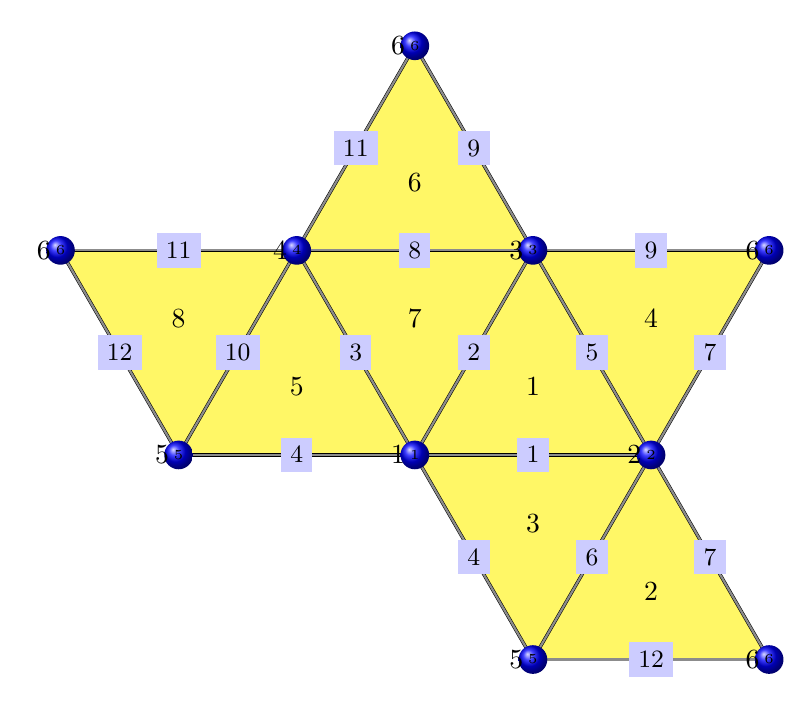
\begin{tikzpicture}[vertexBall, edgeDouble, faceStyle, scale=3]

% Define the coordinates of the vertices
\coordinate (V1_1) at (0, 0);
\coordinate (V2_1) at (1, 0);
\coordinate (V3_1) at (0.5, 0.8660254037844386);
\coordinate (V4_1) at (-0.4999999999999999, 0.8660254037844386);
\coordinate (V5_1) at (0.5, -0.8660254037844386);
\coordinate (V5_2) at (-0.9999999999999998, 1.110223024625157e-16);
\coordinate (V6_1) at (1.5, 0.8660254037844386);
\coordinate (V6_2) at (1.5, -0.8660254037844386);
\coordinate (V6_3) at (5.551115123125783e-17, 1.732050807568877);
\coordinate (V6_4) at (-1.5, 0.8660254037844386);


% Fill in the faces
\fill[face]  (V2_1) -- (V3_1) -- (V1_1) -- cycle;
\node[faceLabel] at (barycentric cs:V2_1=1,V3_1=1,V1_1=1) {$1$};
\fill[face]  (V5_1) -- (V6_2) -- (V2_1) -- cycle;
\node[faceLabel] at (barycentric cs:V5_1=1,V6_2=1,V2_1=1) {$2$};
\fill[face]  (V1_1) -- (V5_1) -- (V2_1) -- cycle;
\node[faceLabel] at (barycentric cs:V1_1=1,V5_1=1,V2_1=1) {$3$};
\fill[face]  (V2_1) -- (V6_1) -- (V3_1) -- cycle;
\node[faceLabel] at (barycentric cs:V2_1=1,V6_1=1,V3_1=1) {$4$};
\fill[face]  (V4_1) -- (V5_2) -- (V1_1) -- cycle;
\node[faceLabel] at (barycentric cs:V4_1=1,V5_2=1,V1_1=1) {$5$};
\fill[face]  (V3_1) -- (V6_3) -- (V4_1) -- cycle;
\node[faceLabel] at (barycentric cs:V3_1=1,V6_3=1,V4_1=1) {$6$};
\fill[face]  (V3_1) -- (V4_1) -- (V1_1) -- cycle;
\node[faceLabel] at (barycentric cs:V3_1=1,V4_1=1,V1_1=1) {$7$};
\fill[face]  (V4_1) -- (V6_4) -- (V5_2) -- cycle;
\node[faceLabel] at (barycentric cs:V4_1=1,V6_4=1,V5_2=1) {$8$};


% Draw the edges
\draw[edge] (V2_1) -- node[edgeLabel] {$1$} (V1_1);
\draw[edge] (V1_1) -- node[edgeLabel] {$2$} (V3_1);
\draw[edge] (V1_1) -- node[edgeLabel] {$3$} (V4_1);
\draw[edge] (V5_1) -- node[edgeLabel] {$4$} (V1_1);
\draw[edge] (V1_1) -- node[edgeLabel] {$4$} (V5_2);
\draw[edge] (V3_1) -- node[edgeLabel] {$5$} (V2_1);
\draw[edge] (V2_1) -- node[edgeLabel] {$6$} (V5_1);
\draw[edge] (V6_1) -- node[edgeLabel] {$7$} (V2_1);
\draw[edge] (V2_1) -- node[edgeLabel] {$7$} (V6_2);
\draw[edge] (V4_1) -- node[edgeLabel] {$8$} (V3_1);
\draw[edge] (V3_1) -- node[edgeLabel] {$9$} (V6_1);
\draw[edge] (V6_3) -- node[edgeLabel] {$9$} (V3_1);
\draw[edge] (V5_2) -- node[edgeLabel] {$10$} (V4_1);
\draw[edge] (V4_1) -- node[edgeLabel] {$11$} (V6_3);
\draw[edge] (V6_4) -- node[edgeLabel] {$11$} (V4_1);
\draw[edge] (V6_2) -- node[edgeLabel] {$12$} (V5_1);
\draw[edge] (V5_2) -- node[edgeLabel] {$12$} (V6_4);


% Draw the vertices
\vertexLabelR[blue]{V1_1}{left}{$1$}
\vertexLabelR[blue]{V2_1}{left}{$2$}
\vertexLabelR[blue]{V3_1}{left}{$3$}
\vertexLabelR[blue]{V4_1}{left}{$4$}
\vertexLabelR[blue]{V5_1}{left}{$5$}
\vertexLabelR[blue]{V5_2}{left}{$5$}
\vertexLabelR[blue]{V6_1}{left}{$6$}
\vertexLabelR[blue]{V6_2}{left}{$6$}
\vertexLabelR[blue]{V6_3}{left}{$6$}
\vertexLabelR[blue]{V6_4}{left}{$6$}

\end{tikzpicture}
\documentclass[12pt,titlepage]{article}
\usepackage[ngerman]{babel}
\usepackage[utf8]{inputenc}
\usepackage[a4paper,lmargin={4cm},rmargin={2cm},
tmargin={2.5cm},bmargin = {2.5cm}]{geometry}
\usepackage{amsmath}
\usepackage{amssymb}
\usepackage{amsthm}
\usepackage{cleveref}
\usepackage{enumerate}
\usepackage{thmtools}
\linespread{1.25}
\usepackage{color}
\usepackage{verbatim}
\newcommand{\gelb}{0.550000011920929}
\usepackage{pgf,tikz,pgfplots}
\pgfplotsset{compat=1.15}
\usepackage{mathrsfs}
\usetikzlibrary{arrows}
%\usepackage{scrheadings}
\pagestyle{headings}
\usepackage{titlesec}                % für Kontrolle der Abschnittüberschriften
\declaretheorem[name=Lemma]{lemma}
\declaretheorem[name=Folgerung]{folgerung}
\declaretheorem[name=Beispiel]{bsp}
\declaretheorem[name=Satz]{satz}
\declaretheorem[name=Herleitung]{herleitung}
\declaretheorem[name=Definition]{definition}
\declaretheorem[name=Bemerkung]{bemerkung}

\begin{document}
\thispagestyle{empty}
\pagenumbering{arabic}
%\begin{titlepage}
\noindent\rule{\textwidth}{0.5pt}
\centerline{\textbf{\large{Funkana}}}
\centerline{Reymond Akpanya}
\noindent\rule{\textwidth}{0.5pt}
\newline
%\farb
\section{Kapitel 1}
\subsection{Allgemeine Begriffe}
\begin{definition}[Prähilbertraum]
Sei $H$ ein Vektorraum über $\mathbb{R}$. Es sei Abbildung $\langle \cdot  , \cdot \rangle:H \times H \to \mathbb{R}, (x,y) \mapsto \langle x,y \rangle_H$ erklärt, die folgende Eigenschaften besitzt:
\begin{enumerate}
\item $\forall (x,y) \in H \times H, \forall \alpha \in \mathbb{R}:\langle \alpha x, y \rangle_H = \alpha\langle x, y \rangle_H$ 
\item $\forall (x,y) \in H \times H:\langle x, y \rangle_H=\langle y,x \rangle_H$
\item $\forall x_1,x_2,y \in H:\langle x_1+x_2, y \rangle_H=\langle x_1, y \rangle_H+\langle x_2, y \rangle_H$
\item $\forall x \in H\setminus \{0\}:\langle x, x \rangle_H>0,\langle x, x \rangle_H=0 \Leftrightarrow x=0.$
\end{enumerate}
$(H,\langle \cdot, \cdot \rangle_H)$ heißt Prähilbertraum, die Abbildung $(x,y)\mapsto \langle x, y \rangle_H$ heißt Skalarprodukt. 
\end{definition}
\begin{folgerung}
\begin{itemize}
\item $\langle x,\alpha y \rangle_H=\alpha\langle x, y \rangle_H$
\item $\langle x, y_1+y_2 \rangle_H=\langle x, y_1 \rangle_H+\langle x, y_2 \rangle_H$
\item Aufgabe: zeige, dass $\Vert x \Vert_H=\sqrt{\langle x, x \rangle_H}$ eine Norm ist.
\item Beweise die Parallelogrammeigenschaft:
\[
\Vert x+y \Vert_H^2+\Vert x-y \Vert_H^2=\Vert x \Vert_H^2+\Vert y \Vert_H^2
\]
\end{itemize}
\end{folgerung}
\begin{bsp}
\begin{enumerate}
\item Sei $\Omega\subset \mathbb{R}^n$ eine beschränkte und offene Menge. Definiere auf $C^0(\bar{\Omega})$:
\[
\langle f,g \rangle := \int f(x)g(x)dx
\]
Dann wird $C^0(\bar{\Omega})$ zu einem Prähilbertraum.
\item Sei $\Omega \subset \mathbb{R}^n$ beschränkt, wegzusammenhängend und offen und außerdem $H=\{f \in C^1(\Omega)\mid f_{|\partial \Omega}=0\}$. Dann definere $\langle f,g \rangle:=\int_\Omega \nabla f(x) \nabla g(x)dx$. Dann ist $\Vert f\Vert =\int_\Omega \vert \nabla f(x)\vert^2dx^{\frac{1}{2}}$ und es gilt $\Vert f \Vert =0 \Leftrightarrow \nabla f(x)=0 \Rightarrow f=const \Rightarrow const =0\Rightarrow$ H ist ein Prähilbertraum.
\end{enumerate}
\end{bsp}
\begin{definition}
Ein Prähilbertraum $H$ heißt Hilbertraum, wenn der normierte Raum $(H,\Vert \cdot Vert_H)$ vollständig ist, d.h. wenn jede Cauchy-Folge in $H$ Grenzwert in $H$ hat.
\end{definition}
\begin{bsp}
Es sei $l_2:=\{a=(a_n)_n \mid a_n \in \mathbb{R}, \sum_{n=1}^{\infty} konvergiert \}$. Wir definieren die Addition und die skalare Multiplikation auf $l_2$ durch 
\[
a+b:=(a_n+b_n)_n \qquad a,b \in l_2
\]
und 
\[
\alpha \cdot a:= (\alpha\cdot a_n)_n \qquad \alpha \in \mathbb{R}
\]
Damit wird $l_2$ zu einem reellen Vektorraum. Durch $\langle  a,b\rangle_{l_2}:= \sum_{n=1}^{\infty}a_nb_n$ definieren wir ein Skalarprodukt auf $l_2$.Dies induziert durch $\Vert a \Vert_{l_2}::=\sqrt{\langle  a,a\rangle_{l_2}}$ eine Norm auf $l_2$.\\
Ist $l_2$ bezüglich $\Vert \cdot \Vert_{l_2}$ vollständig? $\rightarrow$ Übung $\Rightarrow$ $l_2$ ist ein Hilbertraum.
\end{bsp}
\begin{bemerkung}
Es sei $B_1(0)=\{x\in \mathbb{R}^n\mid \Vert x \Vert \leq 1\}$. Dann ist $\bar{B_1(0)}$ kompakt in $\mathbb{R}^n$. In $\infty$-dimensionalen Räumen ist dies im Allgemeinen falsch. Die Einheitskugel in $l_2$ ist nicht kompakt. Warum nicht? Als normierter Raum ist $l_2$ auch ein metrischer Raum. Deshalb gilt $K \subset l_2$ kompakt $\Leftrightarrow$ $K$ ist folgenkompakt $\Leftrightarrow $ jede Folge in $K$ hat eine konvergente Teilfolge.
Setze $a^k=(a^k_n)_n$ mit $a^k_n=
 \left\{
\begin{array}{ll}
1 & k =n \\
0 & k \neq n \\
\end{array}
\right.$ . Rechne $\Vert a^k \Vert_{l_2} =1 \Rightarrow a^k \in K$ für alle $K\in \mathbb{N}$. Für $k\neq l$ gilt $\Vert a^k-a^l \Vert_{l_2}=(1+1)^{\frac{1}{2}}=\sqrt{2} \Rightarrow (a^k)_n \subset l_2$ besitzt keinen Häufungspunkt in $K$. Also lässt sich keine konvergente Teilfolge auswählen. Somit ist $K$ nicht folgenkompakt und damit ebenfalls nicht kompakt.
\end{bemerkung}
\begin{definition}{Orthonormalsystem}
Es sei $H$ ein Prähilbertraum. Ein endliches oder abzählbar unendliches System $\{\phi_1,\phi_2,\ldots\}\subset H$ heißt orthonormiert, falls $\langle \phi_i,\phi_j \rangle_H= \delta_{ij}$ ist.
\end{definition}
\begin{definition}
Es sein $H$ ein Prähilbertraum. Es sei $\{\phi_1,\phi_2,\ldots\}\subset H$ ein Orthonormalsystem. Dann heißt $f_k:=\langle f, \phi_k\rangle_H$ der $k-te$ Fourierkoeffizient von $f$.
\end{definition}
 \begin{bsp}
 Sei $L^2(-\pi, \pi)$ der Raum aller $p-$mal Lebesgue-integrierbaren Funktion auf $(-\pi,\pi)$. Dies ist ein reeller Vektorraum mit dem Skalarprodukt $\langle f, g\rangle:=\int_{-\pi}^\pi f(x)g(x)dx$. Betrachte die Familie
 $\{1\} \cup \{sin(nx),cos(nx)\mid n \in \mathbb{N}\}$. die Funktionen sind in $L^2$. Was ist mit dem Skalarprodukt im Hinblick auf Definition $\textcolor{red}{1.1.6}$?
 \begin{itemize}
 \item $\langle 1,cos(nx) \rangle=\int_{-\pi}^\pi cos(nx)dx=\frac{1}{n}sin(nx)|_{-\pi}^\pi=0$
 \item $\langle 1,sin(nx) \rangle=\int_{-\pi}^\pi sin(nx)dx=\frac{1}{n}cos(nx)|_{-\pi}^\pi=0$
 \item \begin{align*}
 \langle cos(nx),cos(mx) \rangle&=\int_{-\pi}^\pi cos(nx)cos(mx)dx\\
 &=\int_{-\pi}^\pi\frac{1}{2}cos((n-m)x)+\frac{1}{2}cos((n+m)x)dx\\
& \overset{n \neq m}{=} \frac{1}{2}[\frac{1}{n-m}sin((n-m)x)+\frac{1}{n+m}sin((n+m)x)]_{-\pi}^\pi=0
 \end{align*}
 Ähnlich zeigt man $0=\langle sin(nx), sin(mx)\rangle \overset{n\neq m }{=} \langle sin(nx),cos(mx)\rangle.$
 \end{itemize}
 Beachte nun, dass
 \begin{itemize}
\item $\Vert 1 \Vert_{L^2}^2=2\pi $,
 \item $\Vert cos(nx) \Vert_{L^2}^2=\int_{-\pi}^\pi cos^2(nx)dx=\int_{-\pi}^\pi \frac{1}{2}(1+cos(2nx))dx =\pi$,
 \item  $\Vert sin(nx) \Vert_{L^2}^2=\int_{-\pi}^\pi \frac{1}{2}(1-cos(2nx))dx =\pi$ ist.
 \end{itemize} 
 Normiert man nun, so erhält man das Orthonormalsystem $\{\frac{1}{\sqrt{2}}\}\cup \{\frac{1}{\sqrt{\pi}}cos(nx),\frac{1}{\sqrt{\pi}}sin(nx)\mid n \in \mathbb{N}\}$ im Sinne von Definition $\textcolor{red}{1.1.6}$.
 \end{bsp}
 \begin{satz}
 Es sei $H$ ein Prähilbertraum und $f \in H$. Es seien $\phi_1,\ldots,\phi_N \in H$ orthonormiert und $c_1 \ldots C_N \in \mathbb{R}$. Setze nun $f_k=\langle f, \phi_k\rangle_H$ für $k=1,\ldots N$. Dan gilt:
 \begin{enumerate}
 \item $\Vert f- \sum_{k=1}^Nf_k\phi_k\Vert_H^2=\Vert f\Vert_H^2- \sum_{k=1}^N \vert f_k\vert^2$
 \item $\Vert f- \sum_{k=1}^Nc_k\phi_k\Vert_H^2=\Vert f\Vert_{H}^2-\sum_{k=1}^N \vert f_k\vert^2+\sum_{k=1}^N \vert c_k- f_k\vert^2$
 \end{enumerate}
 \end{satz}
 \begin{bemerkung}
 Insbesondere besagt $(2)$, dass die Approximation von $f$ durch Linearkombination der $\phi_1, \ldots \phi_N$ bestmödlich ist, wenn die Koeffizienten $c_i$ gerade die Fourierkoeffizienten sind
  \end{bemerkung}
  \begin{satz}[Besselsche Ungleichung]
  Es sei $H$ ein Prähilbertraum und $\{\phi_1,\phi_2, \ldots\}$ ein Orthonormalsystem. Dann ist $\sum_{k=1}^{\infty} \vert f_k \vert^2 \leq \Vert f \Vert_H^2$ und Gleichheit gilt genau dann, wenn $\underset{N\rightarrow \infty}{\lim}\Vert f-\sum_{k=1}^{N}f_k \phi_k\Vert=0 ist, d.h. f= \sum_{k=1}^{\infty}f_k \phi_k$
  \end{satz}
  \begin{proof}
  Nutze $(1)$ aus $\textcolor{red}{1.1.9}$:
  \[
0\leq   \Vert f- \sum_{k=1}^N f_k\phi_k\Vert^2= \Vert f \Vert^2-\sum_{k=1}^{N} \vert f_k \vert^2
  \]
  Also gilt für alle $n \in \mathbb{N}:$
  \[
  \sum_{k=1}^{N} \vert f_k \vert^2 \leq \Vert f \Vert^2.
  \]
  D.h. die Reihe konvergiert und die Ungleichung im Satz gilt. Außerdem ist \begin{align*}
  &\Vert f \Vert^2=\underset{N \Rightarrow \infty}{\lim}\sum_{k=1}^N\\
  \overset{\textcolor{red}{1.1.9}}{\Leftrightarrow}& \Vert f- \sum_{k=1}^Nf_k\phi_k \Vert^2=0\\
 \Leftrightarrow &f=\sum_{k=1}^{\infty}f_k\phi_k
  \end{align*}
   \end{proof}
 \begin{definition}[vollst. Orthogonalsystem]
 Sei $H$ ein Prähilbertraum. Ein Orthogonalsystem $(\phi_1,\phi_2, \ldots)$ heißt vollständig in $H$ genau dann, wenn für jedes $f \in H$ gilt: $\sum_{k=1}^{\infty}\vert f_k\vert^2=\Vert f \Vert^2=\langle f,f \rangle.$
 \end{definition}
 \begin{bsp}
 Die orthonormierte Familie $\{\frac{1}{\sqrt{2}}\}\cup \{\frac{1}{\sqrt{\pi}}cos(nx),\frac{1}{\sqrt{\pi}}sin(nx)\mid n \in \mathbb{N}\}$ ist ein VONS für $L^2((-\pi,\pi))=\{f:(-\pi,\pi)\to \mathbb{R} \mid f \, messbar, \int_{-\pi}^\pi \vert f \vert^2 < \infty\}$. Der Beweis kann jetzt noch nicht geführt werden.
 \end{bsp}
\begin{bemerkung}
Es sei $H$ ein Prähilbertraum und $(\phi_1,\phi_2,\ldots)$ sei ein Orthonormalsystem. Dann gilt: $(\phi_1,\phi_2,\ldots)$ ist vollständig $\Leftrightarrow$ Zu jedem $f\in H$ und jedem $\epsilon>0 $ gibt es ein $N(\epsilon,f) \in \mathbb{N}$ und $c_1 ,\ldots,c_N$, so dass $ \Vert f- \sum_{k=1}^N c_kf_k \Vert <\epsilon$
\end{bemerkung}
\begin{proof}
"$\Rightarrow$" Wähle $c_k=f_k$\\
"$\Leftarrow$" Nach $\textcolor{red}{1.1.9}$ folgt $\Vert f \Vert^2=\sum_{k=1}^{\infty}\vert f_k\vert^2 $. Das liefert die Vollständigkeit.
\end{proof}
\begin{satz}[Cauchy-Ungleichung]
Es sei $H$ ein Prähilbertraum und es seien $f,g \in H$. Dann gilt 
\[
\vert \langle f,g \rangle\vert \leq \Vert f \vert \Vert g\Vert.
\]
\end{satz}
\begin{proof}
Siehe Aufgabe 4 Blatt 1
\end{proof}
\begin{bemerkung}
Es sei $H$ ein Prähilbertraum und $x_n,x,y_n,y\in H$ für $n\in \mathbb{N}$.
\begin{enumerate}
\item  Die folgenden Aussagen sind äquivalent:
\begin{itemize}
\item $\underset{n \rightarrow \infty}{\lim} x_n=x$
\item $\underset{n \rightarrow \infty}{\lim} \Vert x_n \Vert =\Vert x \Vert$ und für alle $y\in H$ gilt $\underset{n \rightarrow \infty}{\lim} \langle x_n,y \rangle= \langle x,y \rangle$
\end{itemize}
\item Es sei $\underset{n \rightarrow \infty}{\lim} x_n =x$ und $\underset{n \rightarrow \infty}{\lim} y_n=y$. Dann gilt auch $\underset{n \rightarrow \infty}{\lim} \langle x_n, y_n \rangle = \langle x,y \rangle.$
\end{enumerate}
\end{bemerkung}
 %\docite{*}\bibliography{literatur}
%\bibliographystyle{plain}
\end{document};
\end{document}
